\documentclass[twoside]{article}

\usepackage{aistats2023}
% If your paper is accepted, change the options for the package
% aistats2023 as follows:
%
%\usepackage[accepted]{aistats2023}
%
% This option will print headings for the title of your paper and
% headings for the authors names, plus a copyright note at the end of
% the first column of the first page.

% If you set papersize explicitly, activate the following three lines:
%\special{papersize = 8.5in, 11in}
%\setlength{\pdfpageheight}{11in}
%\setlength{\pdfpagewidth}{8.5in}

% If you use natbib package, activate the following three lines:
\usepackage[round]{natbib}
\renewcommand{\bibname}{References}
\renewcommand{\bibsection}{\subsubsection*{\bibname}}
\bibliographystyle{plainnat}
\usepackage{amsmath}
\usepackage{amssymb}
\usepackage{hyperref}
\usepackage{graphicx}
\graphicspath{ {./../examples/} }
% If you use BibTeX in apalike style, activate the following line:
%\bibliographystyle{apalike}

\newcommand{\dfdx}{\frac{\partial f}{\partial x_s}}
\newcommand{\xc}{\mathbf{x_c}}
\newcommand{\DY}{\mathbf{\Delta Y}}
\newcommand{\xb}{\mathbf{x}}
\newcommand{\Xcb}{\mathbf{X}_c}
\newcommand{\Xb}{\mathcal{X}}

\begin{document}

% If your paper is accepted and the title of your paper is very long,
% the style will print as headings an error message. Use the following
% command to supply a shorter title of your paper so that it can be
% used as headings.
%
%\runningtitle{I use this title instead because the last one was very long}

% If your paper is accepted and the number of authors is large, the
% style will print as headings an error message. Use the following
% command to supply a shorter version of the authors names so that
% they can be used as headings (for example, use only the surnames)
%
%\runningauthor{Surname 1, Surname 2, Surname 3, ...., Surname n}

\twocolumn[

\aistatstitle{Instructions for Paper Submissions to AISTATS 2023}

\aistatsauthor{ Author 1 \And Author 2 \And  Author 3 }

\aistatsaddress{ Institution 1 \And  Institution 2 \And Institution 3 } ]

\begin{abstract}
  The Abstract paragraph should be indented 0.25 inch (1.5 picas) on
  both left and right-hand margins. Use 10~point type, with a vertical
  spacing of 11~points. The \textbf{Abstract} heading must be centered,
  bold, and in point size 12. Two line spaces precede the
  Abstract. The Abstract must be limited to one paragraph.
\end{abstract}


\section{INTRODUCTION}

Recently, ML has flourished in critical domains, such as healthcare
and finance. In these areas, we need ML system with the capability to
explain their predictions, apart from predicting with accuracy. For
this reason there is an increased interest in Explainable AI (XAI),
the field that provides interpretations about the behavior of complex
black-box models. XAI literature distinguishes between local and
global explainability
techniques~\citep{Molnar2020interpretable}. Local methods explain a
specific prediction, whereas global methods explain the entire model
behavior. Global methods provide a universal explanation, summarizing
the numerous local ones into a single interpretable outcome, usually a
number or a plot. If a user wants to get a rough overview about which
features are significant (feature importance) or whether a particular
feature has a positive or negative effect on the output (feature
effect), they should opt for a global explainability technique. On
the other hand, aggregating the individual explanations for producing
a concise global one is vulnerable to misinterpretations; Under strong
feature interactions, the global explanation may obfuscate
heterogeneous effects~\citep{Herbinger2022repid} that exist under the
hood; a phenomenon called aggregation bias~\citep{mehrabi2021survey}.

Feature effect (FE) \citep{Gromping2020MAEP} is a fundamental category
of global explainability methods. The objective of FE is to the
isolate and visualize the impact of a single feature on the
output.~\footnote{FE methods also isolate the effect of a pair of
  features to the output. Combinations of more than two features are
  not usual, because they encounter, among others, visualization
  difficulties.} FE methods suffer from aggregation bias because,
often, the rationale behind the average effect might be unclear. For
example, a feature with zero average effect may indicate that the
feature has no effect on the output or, contrarily, it has a highly
positive effect in some cases and a highly negative in others. There
are three widely-used FE methods; Partial Dependence Plots
(PDP)\citep{friedman2001greedy}, Marignal Plots
(MP)\citep{apley2020visualizing} and Aggregated Local Effects
(ALE)\citep{apley2020visualizing}. PDP and MP have been criticized for
computing erroneous effects when the input features are (highly)
correlated, which is a frequent scenario in many ML
problems. Therefore, ALE has been established as the state-of-the-art
FE method.

However, ALE faces two crucial drawbacks. First, it does not inform
the user about potential heterogeneous effects hidden behind the
average effect. In contrast, in the case of PDP, the heterogeneous
effects can be spotted by exploring the Individual Conditional
Expectations (ICE)\citep{goldstein2015peeking}. Second, ALE
approximation from the samples of the training set requires
partitioning the axis of the feature of interest in a sequence of
non-overlapping intervals and estimating a single effect from the
population of samples in each interval. We refer to this step using
the term \textit{bin-splitting problem}. Deciding on the sequence of
intervals has important implications because ALE's interpretation in
cases of correlated features is meaningful only inside each interval
\citep{molnar2022}. However, this crucial step has not been given the
appropriate attention, making the approximation vulnerable to
potential misinterpretations.

In this paper, we extend ALE with a probabilistic component for
measuring the uncertainty of the explanation. The uncertainty of the
global explanation expresses how certain we are that the averaged
explanation is valid if applied to an instance drawn at random and
reveals the heterogeneous effects. Given that ALE's interpretation
(expected effect and uncertainty) is meaningful only inside each
interval, we design a principled framework, where we treat the
bin-splitting step as a data-driven clustering problem, searching for
the optimal splitting given available instances of the training
set. We, also, present a computationally-grounded algorithm for
finding the optimal solution.

\paragraph{Contributions.} The contribution of this paper is NAME, a
feature effect method that:

\begin{itemize}
\item Extends ALE with a probabilistic component to quantify the
  heterogeneous effects behind the global explanation.
\item Automatically extracts regions with similar effects, improving
  the estimation and the interpretability of ALE plots.
\end{itemize}

We provide empirical evaluation of the method in artificial and real
datasets. The implementation of our method and the code for
reproducing all the experiments is provided in the submission and will
become publicly available upon acceptance.


\section{BACKGROUND AND RELATED WORK}

\paragraph{Notation.} We refer to random variables (rv) using
uppercase \( X \), whereas to simple variables with plain lowercase
\( x \). Bold denotes a vector; \( \xb \) for simple variables or
\(\mathbf{X}\) for rvs. Often, we partition the input vector
\(\xb \in \mathbb{R}^D\) to the feature of interest
\(x_s \in \mathbb{R} \) and the rest of the features
\(\xc \in \mathbb{R}^{D-1}\). For convenience we denote it as
\((x_s, \mathbf{x}_c)\), but we clarify that it corresponds to the
vector \((x_1, \cdots , x_s, \cdots, x_D)\). Equivalently, we denote
the corresponding rv as \(X = (X_s, \mathbf{X}_c)\). The black-box
function is \(f : \mathbb{R}^D \rightarrow \mathbb{R}\) and the
FE of the \(s\)-th feature is
\(f^{\mathtt{<method>}}(x_s)\), where \(\mathtt{<method>}\) is the
name of the FE method.\footnote{An extensive list of all
  symbols used in the paper is provided in the helping material.}

\paragraph{Feature Effect Methods.} The three well-known feature
effect methods are: PDP, MP and ALE. PDP formulates the FE
of the \(s\)-th attribute as an expectation over the marginal
distribution \(\mathbf{X}_c\), i.e.,
\(f^{\mathtt{PDP}}(x_s) =
\mathbb{E}_{\mathbf{X}_c}[f(x_s,\mathbf{X}_c)]\), whereas MP
formulates it as an expectation over the conditional
\(\mathbf{X}_c|X_s\), i.e.,
\(f^{\mathtt{MP}}(x_s) = \mathbb{E}_{\mathbf{X}_c|X_s = x_s}[f(x_s,
\mathbf{X}_c)]\). ALE computes the global effect at \(x_s\) as the
accumulation of the averaged local effects:
\begin{equation}
  \label{eq:ALE_accumulated_mean}
  f^{\mathtt{ALE}}(x_s) = \int_{z_{s,min}}^{x_s} \mathbb{E}_{\Xcb|X_s=z}\left[\frac{\partial f(z, \Xcb)}{\partial z}\right] \partial z
\end{equation}
%
ALE has specific advantages which gain particular value in cases of
correlated input features. In these cases, PDP integrates over
unrealistic instances, due to the use of the marginal distribution
\(\mathbf{X}_c \), and MP computes aggregated effects, i.e., imputes
the combined effect of sets of features to a single feature. ALE
manages to resolve both issues, and is therefore a trust able FE method
in cases of correlated features.

\paragraph{Quantify the Heterogeneous Effects.}

FE methods answer the question \textit{what is expected to happen to
  the output (expected effect), if the value of a specific feature is
  increased/decreased}. Having an answer to the question above, it
comes naturally to also wonder \textit{how certain we are about the
  expected change (uncertainty)}. For this reason, the quantification
of the uncertainty along with the expected effect has attracted a lot
of interest. The level of uncertainty is mostly quantified by
measuring the existence of heterogeneous effects, i.e. whether there
are local explanations that deviate from the expected global
effect. ICE and d-ICE plots provide a visual understanding of the
heterogeneous effects on top of PDPs. Another approach targets on
grouping the heterogeneous effects, e.g., allocating ICE plots in
homogeneous clusters, by dividing the input
space.\citep{molnar2020model} Some other approaches, like H-Statistic,
Greenwel, move a step behind and try to quantify the level of
interaction between the input features, a possible cause of
heterogeneous effects. In this case, the interpretation is indirect,
since a strong interaction index is only an indicator of heterogeneous
effects. The aforementioned approaches are under two limitations; They
either do not quantify the uncertainty of the FE directly or they are
based on PDPs, and, therefore, they are subject to the failure modes
of PDPs in cases of correlated features. To the best of our knowledge,
no method so far targets on quantifying the uncertainty of ALE.

\paragraph{Bin-Splitting for ALE estimation.}

In real ML scenarios, the FE is estimated from the limited instances
of the training set.  \citep{apley2020visualizing} proposed dividing
the \(s\)-th axis in \(K\) bins and estimating the local effects in
each bin by evaluating the black box-function at the bin limits:
\begin{equation}
  \label{eq:ALE_accumulated_mean_est}
  \hat{f}^{\mathtt{ALE}}(x_s) = \sum_{k=1}^{k_x} \frac{1}{|\mathcal{S}_k|} \sum_{i:\mathbf{x}^i \in
    \mathcal{S}_k} \left [ f(z_{k}, \xc^i) - f(z_{k-1}, \xc^i)) \right ]
\end{equation}
We denote as \(k_x\) the index of the bin that \(x_s\) belongs to,
i.e. \(k_x: z_{k_x-1} \leq x_s < z_{k_x} \) and \(\mathcal{S}_k\) is
the set of training instance that lie in the \(k\)-th bin, i.e.
\( \mathcal{S}_k = \{ \xb^i : z_{k-1} \leq x^i_s < z_{k} \}
\). Afterwards, (cite) proposed the Differential ALE (DALE) for
computing the local effects on the training instances using auto-differentiation:
\begin{equation}
  \label{eq:DALE_accumulated_mean_est}
  \hat{f}^{\mathtt{DALE}}(x_s) = \Delta x \sum_{k=1}^{k_x} \frac{1}{|\mathcal{S}_k|} \sum_{i:\mathbf{x}^i \in
    \mathcal{S}_k} \frac{\partial f}{\partial x_s}(\mathbf{x}^i)
\end{equation}
%
Their method has the advantages of remaining on-distribution even when
bins become wider and, most importantly, allows the recomputation of
the accumulated effect with different bin-splitting with near-zero
computational cost. However, none of the approximations above deals
with the crucial problem of bin-splitting. As indicated
by~\citep{molnar2022}, in ALE the effects are computed per interval
(region) and the interpretation of the effect can only be
local.


\section{THE NAME METHOD}
\label{sec:NAME-method}

The NAME method extends ALE for measuring the uncertainty of the
expected effect and automatically extracts regions with homogeneous
effects. In Section~\ref{sec:NAME-definition} we define the component
for the uncertainty quantification. In
Section~\ref{sec:interval-based-estimation}, we show how to estimate
the average effect and the uncertainty on a specific interval from the
limited samples of the training set. We, also, make an important proof
about the aggregated variance defined over a bin. In
Section~\ref{sec:interval-spliting}, we define and solve the problem
of optimal bin-splitting for automatically extract regions with
homogeneous effects. Finally, in Section~\ref{sec:visualization}, we
illustrate the appropriate visualization of NAME for facilitating its
interpretation by a non-expert and we discuss important aspects of the
method.

\subsection{Uncertainty Quantification}
\label{sec:NAME-definition}

ALE defines the local effect of the \(s\)-th feature at point
\((x_s, \xc)\) as \(\dfdx (x_s, \xc)\). All the local explanations at
\(x_s\) are, then, weighted by the conditional distribution
\(p(\xc|x_s)\) and are averaged, to produce the summarized effect at
\(x_s\):
\begin{equation}
  \label{eq:ALE_mean}
  \mu(x_s) = \mathbb{E}_{\Xcb|x_s}\left [\dfdx (x_s, \Xcb)\right ]
\end{equation}
%
The FE at \(x_s\) is the accumulation of the averaged local effects
from \(x_{s, min}\)\footnote{\(x_{s,min}\) is the minimum value the
  \(s\)-th attribute can take. In estimations, it is the minimum
  \(s\)-th attribute value among the training set instances.} until
\(x_s\), i.e.
\(f^{\mathtt{ALE}}(x_s) = \int_{x_{s, min}}^{x_s} \mu(z) \partial z
\). Limiting the explanation to the expected value level does not
shed light to potential heterogeneous effects behind the averaged
explanation. Therefore, we model the uncertainty of the local effects
\(\mathcal{H}(x_s)\) with the variance of the local explanations:
\begin{equation}
  \label{eq:ALE_var}
  \mathcal{H}(x_s) := \sigma^2(x_s) = \mathrm{Var}_{\Xcb|x_s}\left [\dfdx (x_s, \Xcb) \right ]
\end{equation}
\noindent
The uncertainty of the explanation emerges from the natural
characteristics of the experiment, i.e.,~the data generating
distribution and the properties of the black-box function. In
Section~\ref{sec:visualization}, we propose appropriate visualizations
for easier interpretation of Eq.~(\ref{eq:ALE_var}). ALE defines the
FE at \(x_s\) as the accumulation of the averaged local effects from
\(x_{min}\) until \(x_s\). Equivalently, we define the accumulated
uncertainty (variance) until \(x_s\), as the integral of the variances
of the local effects:
\begin{equation}
  \label{eq:ALE_accumulated_var}
  f^{\mathtt{ALE}}_{\sigma^2}(x_s) = \int_{z_{s, min}}^{x_s} \sigma^2(z) \partial z
\end{equation}
\noindent
The accumulated uncertainty is not a directly interpretable quantity,
since it measures the total uncertainty that characterizes the
\(s\)-th feature effect plot. As stated in the Introduction, ALE
outcomes should be interpreted at a local level, therefore, the only
\(\mathcal{H}(x_s)\) is the directly interpretable quantity. However,
the accumulated uncertainty will help us define a sensible objective
for the bin-splitting step, as we will discuss in
Section~\ref{sec:interval-spliting}.

\subsection{Interval-Based Estimation}
\label{sec:interval-based-estimation}

In real scenarios, we have ignorance about the data-generating
distribution \(p(x_s, \mathbf{x}_c)\), so, the estimations are based
on the limited instances of the training set. Estimating
Eqs.~\eqref{eq:ALE_mean},~\eqref{eq:ALE_var} at the granularity of a
point is impossible, because the probability of observing a sample
inside the interval \([x_s - h, x_s + h]\) tends to zero, when
\(h \to 0\). We are, therefore, obliged to split the axis of \(x_s\)
into a sequence of non-overlapping intervals (bins) and estimate the
mean and the variance from the samples that lie inside each bin. The
mean effect at an interval \([z_1, z_2)\) is defined as the mean of
the expected effects:
\begin{equation}
  \label{eq:mu_bin}
  \mu(z_1, z_2) = \frac{1}{z_2 - z_1} \int_{z_1}^{z_2}
  \mathbb{E}_{\xc|x_s=z}\left [\frac{\partial f}{\partial x_s} \right ] \partial z
\end{equation}
\noindent
Similarly, the accumulated variance at an interval \([z_1, z_2)\) is
defined as:
\begin{equation}
  \label{eq:var_bin}
  \sigma^2(z_1, z_2) = \int_{z_1}^{z_2}
  \mathbb{E}_{\xc|x_s=z} \left [ (\frac{\partial
      f}{\partial x_s} - \mu(z_1, z_2) )^2 \right] \partial z
\end{equation}
\paragraph{Theorem 1.} If we define the residual \(\rho(z)\) as the
difference between the expected effect at \(x_s\) and the mean
expected effect at the interval, i.e
\(\rho(z) = \mu(z) - \mu(z_1, z_2)\), then, the accumulated variance
\(\sigma^2(z_1, z_2)\) equals to the accumulation of the point-wise
variances plus the squared residuals inside the interval:
\begin{equation}
 \sigma^2(z_1, z_2) = \int_{z_1}^{z_2} \sigma^2(z) + \rho^2(z) \partial z
\end{equation}
%
The proof is in the Appendix. Theorem 1 decouples the total
uncertainty inside a bin
\(\mathcal{H}_{bin}(z_1, z_2) := \sigma^2(z_1, z_2)\) into two terms. The first term quantifies
the accumulated uncertainty due to the natural characteristics of the
experiment, i.e.,
\(\mathcal{H}(z_1, z_2) = \int_{z_1}^{z_2}\mathcal{H}(z) \partial z\),
and the second term adds extra nuisance uncertainty due to limiting
the resolution
\(\mathcal{H}_n(z_1, z_2) := \int_{z_1}^{z_2}\rho^2(z) \partial z
\). In other words, the creation of a bin burdens the estimation with
a nuisance uncertainty:
\begin{equation}
  \label{eq:uncertainty_bin}
  \mathcal{H}_{bin}(z_1, z_2) = \mathcal{H}(z_1, z_2) + \mathcal{H}_n(z_1, z_2)
\end{equation}
Eqs.~\eqref{eq:mu_bin},~\eqref{eq:var_bin} can be directly estimated
from the set \(\mathcal{S}\) of the dataset instances with the
\(s\)-th feature lying inside the interval, i.e.,
\( \mathcal{S}= \{ \mathbf{x}^i : z_1 \leq x^i_s < z_2 \} \). The mean
effect at the interval, Eq.~(\ref{eq:mu_bin}) is approximated by:
\begin{equation}
  \label{eq:mean_estimation}
  \hat{\mu}(z_1, z_2) = \frac{1}{|\mathcal{S}|} \sum_{i:\mathbf{x}^i \in
    \mathcal{S}} \left [ \dfdx(\mathbf{x}^i) \right ]
\end{equation}

and the accumulated variance, Eq.~(\ref{eq:var_bin}) can be
approximated by
\begin{equation}
  \label{eq:variance_estimation}
  \hat{\sigma}^2(z_1, z_2) = \frac{z_2 - z_1}{|\mathcal{S}|} \sum_{i:\mathbf{x}^i \in
    \mathcal{S}} \left ( \dfdx(\mathbf{x}^i) - \hat{\mu}(z_1, z_2) \right )^2
\end{equation}
The approximation is unbiased only if the points are uniformly
distributed in \([z_1, z_2]\). Elaborate.

\subsection{Bin-Splitting: Finding Regions With Homogeneous Effects}
\label{sec:interval-spliting}

As we discussed in the Introduction, when the features are (strongly)
correlated, ALE provides meaningful interpretations only inside a
bin. The accumulation of the mean effects inside each bin is done only
for a producing smooth curve for easier visual exploration. Therefore,
the extraction of regions with common effects is particularly
important for a correct interpretation.

We formulate the bin-splitting as an unsupervised clustering
problem. We want to partition the axis of the \(s\)-th feature into a
sequence of variable-size non-overlapping intervals, so that the
regions that will be created to provide meaningful explanations. A
region with a meaningful explanation means that it clusters together
points with similar expected (averaged) effects. On the other hand,
since we estimate all the quantities from the limited samples of the
training set, we need enough samples inside each bin for robustly
estimate the expected effect and the variance. Therefore, we transform
the bin-splitting problem to the following optimization problem:
\begin{equation}
  \label{eq:opt}
\begin{aligned}
  \min_{ \{z_0, \ldots, z_K\}} \quad & \mathcal{L} = \sum_{k=1}^K \hat{\sigma}^2(z_{k-1}, z_k) \\
  \textrm{s.t.} \quad & |\mathcal{S}_k| \geq N\\
                                     & z_0 = x_{s,min}\\
                                     & z_K = x_{s, max}
\end{aligned}
\end{equation}
%
We search for the sequence of intervals \(z_0, \ldots, z_K\) covering
the axis of the \(s\)-th feature, \(z_0 = x_{s,min}, z_K = x_{s,max}\)
that minimize the sum of bin variances. The constraint of at least
\(N\) points in each bin sets the limit for the minimum number of
points inside each bin, to robustly estimate the mean effect and the
variance. There is no constraint about the bin size and the number of
bins \(K\).

The objective function is the sum of the approximations of the bin
variances. As we prove in Theorem 1, the observable bin variance can
can be split in the accumulation of point-wise variances plus the
residuals. In Corollary 1, we show that the accumulation of the
point-wise variances is independent of the bin-splitting
procedure. Therefore by minimizing \(L\), we minimize the accumulation
of the point-wise residuals in each bin, searching for bins that
cluster together points with a common expected effect. An additional
interpretation is that we search for the bin-splitting that adds the
minimum the nuisance uncertainty over the lower-bound of the
uncertainty due to the natural characteristics of the experiment.

\subsubsection{Solve Bin-Splitting with Dynamic Programming}
\label{sec:dynamic-programing}

For achieving a computationally-grounded solution we set a threshold
\(K_{max}\) on the maximum number of bins which also discretizes the
solution space. The width of the bin can take discrete values that are
multiple of the minimum step
\(u = \frac{x_{s, max} - x_{s, min}}{K}\). For defining the solution,
we use two indexes. The index \(i \in \{0, \ldots, K_{max}\}\) denotes
the \(i\)-th limit \((z_i)\) and the index
\(j \in \{0, \ldots, K_{max}\} \) denotes the \(j\)-th position along
the axis \((x_j = x_{s,min} + j \cdot u)\). The recursive cost
function \(T(i,j)\) is the cost of setting the \(i\)-th limit \(z_i\)
to \(x_j\):
\begin{equation}
  \label{eq:recursive_cost}
  \mathcal{T}(i,j) = \mathrm{min}_{l \in \{0, \ldots, K_{max}\}} \left [ \mathcal{T}(i-1, l) + \mathcal{B}(x_l, x_j) \right ]
\end{equation}
%
where \(\mathcal{T}(0,j)\) equals zero if \(j=0\) and \(\infty\) in
any other case. \(\mathcal{B}(x_l, x_j)\) denotes the cost of creating a bin
with limits \([x_l, x_j)]\):

\begin{equation}
  \label{eq:cost_step}
  \mathcal{B}(x_l, x_j) = \begin{cases}
                            \infty, & \text{if $x_j > x_l$ or \(|\mathcal{S}_{(x_j, x_l)}| < N\)}\\
                            0, & \text{if $x_j = x_l$}\\
                            \hat{\sigma}^2(x_j, x_l), &\text{if $x_j \leq x_l$}
  \end{cases}
\end{equation}

The optimal solution is given by solving
\(\mathcal{L} = \mathcal{T}(K_{max}, K_{max})\) and keeping track of the sequence of
steps. 

% \begin{equation}
%   \label{eq:1}
%   \mathcal{L} = \sum_{k=0}^K \hat{\sigma}_k(z_{k-1}, z_k)
% \end{equation}
% %
% The constraints are that all bins must include more than \(\tau\)
% points, i.e., \(|\mathcal{S}_k| \geq \tau\).

% \(\mathcal{L} = \sum_{k=1}^K \hat{\sigma}^2(z_{k-1}, z_k)\) is the sum
% of the uncertainty of the local explanations \(\mathcal{H}\) due to
% heterogeneous effects and the added nuisance uncertainty due to
% bin-splitting \(\mathcal{H}_n\). Given that \(\mathcal{H}\) is not
% affected by interval splitting, optimizing \(\mathcal{L}\) equals to
% finding the sequence of non-overlaping bins that add the minimum
% nuisance uncertainty. The restriction of (\ref{eq:opt}) secures that
% each bin is populated with enough samples for a robust estimation,
% which is set by the parameter \(N\). In other words, the user makes
% the following proposal; \textit{find the bin sequence that adds the
%   minimum nuisance uncertainty, given that I want at least \(N\)
%   points per bin}.

\noindent

\begin{itemize}
\item Computational complexity
\end{itemize}

\subsection{Visualization and Interpretation}
\label{sec:visualization}

\begin{itemize}
\item Discuss about the meaning of ALE, to find intervals with some effect
\end{itemize}

\clearpage
\section{EXPERIMENTS}

The experimental section is divided in simulation and real-world
examples. The simulation examples, where the data-generating
distribution \(p(\mathbf{X})\) and the predictive function
\(f(\cdot)\) are defined by us, are used for comparing all methods
against a solid ground-truth. Having the freedom to experiment with
\(p(\mathbf{X}), f(\cdot)\), we explore the behavior of each method in
different settings for highlighting important aspects
(advantages/disadvantages) of each one. In particular, we design two
end-to-end simulation examples; At the first one, we focus on
comparing NAME method versus PDP-ICE in terms of quantifying the
heterogeneous effects for a range of different black-box functions. At
the second one, we provide empirical clues that NAME method achieves a
better approximation compared to traditional ALE, due to appropriate
bin-splitting. Afterwards, we also apply the methods on some
real-world datasets. In these cases, it is infeasible to obtain ground
truth information, therefore, we perform evaluation at two
levels. First, we compare visually NAME versus PDP with ICE
plots. Second, we hold as ground-truth the effects computed on the
full training-set and we, then, perform subsampling to evaluate the
robustness of the bin-splitting method.

\paragraph{Metrics.} Describe the metrics used for comparing methods.

\subsection{Synthetic Example 1: Uncertainty Quantification}

In general, there is no a single unchallenged aggreement about the
correct feature effect; each method models it in a slightly different
way. Therefore, for creating a universal evaluation framework we
reside on variations of the simple piecewise-linear function, where in
most cases, we can have an homophony about the correct effect.


In all the experiments of the example, we will use the following
generative distribution: \(p(\mathbf{x}) = p(x_3)p(x_2|x_1)p(x_1)\)
where \(x_1 \sim \mathcal{U}(0,1)\),
\(x_2 \sim \mathcal{N}(x_1, \sigma_2^2)\),
\(x_3 \sim \mathcal{N}(0, \sigma_3^2)\). 
%
The predictive function is:

\begin{equation}
  \label{eq:2}
  f(\mathbf{x}) = \begin{cases}
                    f_{\mathtt{lin}} + \alpha f_{\mathtt{int}} & \text{if $f_{\mathtt{lin}} < 0.5$ }\\
                    0.5 - f_{\mathtt{lin}} + \alpha f_{\mathtt{int}} & \text{if $0.5 \leq f_{\mathtt{lin}} < 1$}\\
                    \alpha f_{\mathtt{int}} &\text{otherwise}
                  \end{cases}
\end{equation}
%
where \(f_{\mathtt{lin}}(\mathbf{x}) = a_1 x_1 + a_2 x_2\) and
\(f_{inter}(\mathbf{x}) = x_1x_3\). The term \(f_{\mathtt{lin}}\) is a
linear function with \(a_1, a_2\) the weights of the corresponding
variables. The term \(f_{\mathtt{lin}}\) is the interaction between
the independent variables \(x_1\) and \(x_3\), with \(\alpha\) setting
the weight of the interaction term.

\subsubsection{Effect Without Uncertainty}

We test the feature effect when no interaction term is apparent,
i.e. \(\alpha=0\), there is no uncertainty about the value of \(x_2\),
i.e. \(x_2 = x_1\) and the weights are equal weights \(a_1=a_2=1\).
In this case, ground truth effect for \(f^{\mathtt{GT}}(x_1)\) is
\(x_1\) when \(0 \leq x_1 < 0.25\), \(-x_1\) when
\(0.25 \leq x_1 < 0.5\) and zero otherwise. In each position \(x_1\),
there is complete absence of heterogeneous effects, and therefore, the
uncertainty of the global explanation is zero,
i.e. \(f^{\mathcal{GT}}_{\sigma^2}(x_1) = 0\). In figure we present,
the effect of each method;

\begin{figure}[h]
  \centering
  \includegraphics[width=.23\textwidth]{example_3/dale_auto_bins.png}
  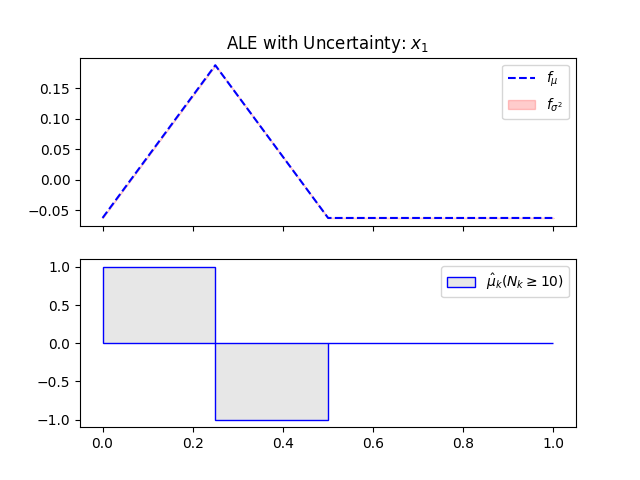
\includegraphics[width=.23\textwidth]{example_3/pdp_ice.png}
  \caption{Figure 1}
  \label{fig:ex-synth-1-1}
\end{figure}

\subsubsection{Effect With Uncertainty}




\subsection{Synthetic Example 2: Bin-Splitting}

The perfect bin-splitting according to the definition of the
minimization problem, is the one that creates:

\begin{itemize}
\item the biggest bins in regions with constant effect
\item the smallest bins with \(N_k > \tau\), in regions with non-constant effect
\end{itemize}

Prove that (a) this is a good objective, i.e., prove that on average,
this splitting gives the minimum distance from the ground truth ALE
and (b) that DP finds the optimal.

Set-ups:

For limited instances, measure the mean error and std (many seeds)
between gt ALE with uncertainty and approximation with bin-splitting
using (a) fixed-size bins (b) variable-size bins for many \(K\)

for many different \(N_k\)

\begin{itemize}
\item In case where the perfect bin-splitting is served by
  equally-sized bins, DP finds it automatically. Without DP, the user
  should try many different \(K\). and compare them the user's overhead of
  testing many differ
\end{itemize}

For many model-agnostic interpretation techniques
– including interaction detection methods – ground
truth information is usually not available on real-world
data. Therefore, well-constructed simulation experi-
ments with a known ground truth are often used for
empirical evaluations and comparisons, while only one
or few real-world datasets are used to demonstrate
practical applicability (e.g., see Friedman et al. (2008),
Fisher et al. (2019), Goldstein et al. (2015), Greenwell
et al. (2018), or Aas et al. (2021)). Hence, we follow
this commonly used approach to evaluate our method
using various simulation settings.

\section{REAL-WORLD EXAMPLES}


\subsubsection*{Acknowledgments}
All acknowledgments go at the end of the paper, including thanks to reviewers who gave useful comments, to colleagues who contributed to the ideas, and to funding agencies and corporate sponsors that provided financial support. 
To preserve the anonymity, please include acknowledgments \emph{only} in the camera-ready papers.

\bibliography{biblio}

\end{document}
